\chapter{Conclusion}

\begin{table}[]
\centering
\caption{Results: the best accuracy of different models}
\label{resultAll}
\begin{tabular}{|c|c|}
\hline
Tf-IDF   & 0.44 (± 0.04) \\
PVDM(dbow) & 0.40    \\
Fasttext &  0.51   \\
Fasttext(Pinyin) &  0.51  \\
Siamese-CBOW(10) with pre-train & 0.45 (± 0.02) \\

\hline
\end{tabular}
\end{table}

\begin{table}[]
\centering
\caption{Fasttext}
\label{fasttext}
\begin{tabular}{|c|c|c|c|c|c|}
\hline
   & 8 & 12 & 16 & 32 & 64 \\
\hline
no segmentation  & 0.369 & 0.375 & 0.389 & 0.372 & 0.368 \\
segmentation  & 0.515 & 0.515 & 0.514 & 0.516 & 0.513 \\
pinyin  & 0.513 & 0.518 & 0.516 & 0.517 & 0.51 \\
\hline
\end{tabular}
\end{table}


\begin{table}[]
\centering
\caption{Results: the accuracy of Siamese-CBOW}
\label{resultSCBOW}
\begin{tabular}{|c|c|}
\hline
Siamese-CBOW(5) & 0.41 (± 0.04) \\
Siamese-CBOW(10) & 0.39 (± 0.03) \\
Siamese-CBOW(10) with pre-train & 0.45 (± 0.02) \\
\hline
\end{tabular}
\end{table}

\begin{table}[]
\centering
\caption{Result of PVDM}
\label{resultPVDM}
\begin{tabular}{|c|c|c|c|}
\hline
      & Test set & Training Set \\
\hline
DM/C  & 0.384 &  0.384 \\
DM/M &  0.38  & 0.436 \\
DBOW &  0.404  & 0.457 \\
\hline
\end{tabular}
\end{table}


\section{Experiment Settings}


We used baseline TD-IDF plus SVM with linear kernel as baseline. 
Since the original distribution for classes is a little skewed, most of the test samples are classified into 2 major classes.
We compared it with other models with different settings. \\

For PVDM, we use 3 different models DM/C, DM/M and DBOW. All of them, we choose most commonly used parameters, DM : dimension:100, window size:10, negative:5, hs:0 and we tested both DM with concatenation of context vectors (DM/C) and average of context vectors(DM/M). 
The other model dbow, we chose the same parameters.

In FastText experiment, we iterated through the parameters like window size from 8 to 100, 
loss function ns, hs, softmax.  Since the result did not indicate significant difference between these parameters, 
we only display 1 of them as reference.

Additionally, we also tried to convert dataset to pinyin to evaluate if pinyin improve the semantic recognition for FastText, 
which support vocabulary expansion with subword information \cite{bojanowski2016enriching}. 

\section{Result}

It took around 2 days with GPU NVIDIA TITAN X (PASCAL) to finish Siamese-CBOW word embeddings training. The perforamance with epoch 5, 10 are below the baseline. 
The other models were finished with CPU within hours.

Figure \ref{resultSCBOW} and Figure \ref{resultPVDM} show the accuracy for Siamese-CBOW and PVBM separately. 
In the experiment of Siamese-CBOW, we found that the result without pre-trained embedding of Siamese-CBOW is below the baseline. We trained the original dataset with Gensim word2vec as pretrained embeddings.
The result is improved by the pre-trained embeddings, but it is not significant statistically from the baseline. In the result of PVDM, DBOW perform better than the other 2 DM models by little. 
The overall accuracy is a little below of baseline.

We also look into the classification result with confusion matrix in Figure \ref{confusion1} and Figure \ref{confusion2}.
That we can see that the 2 major classes give the best accuracy while the test results skewed into these 2 major classes as well.  
The ANGER, DISGUST, and FEAR are more likely to be classified as SAD. It is reasonable that those posts contain more negative sentiment.
The tendency in the Siamese-CBOW result is more obvious. It classify no entry into some rarely used classes.

\begin{figure}[h]
    \centering
	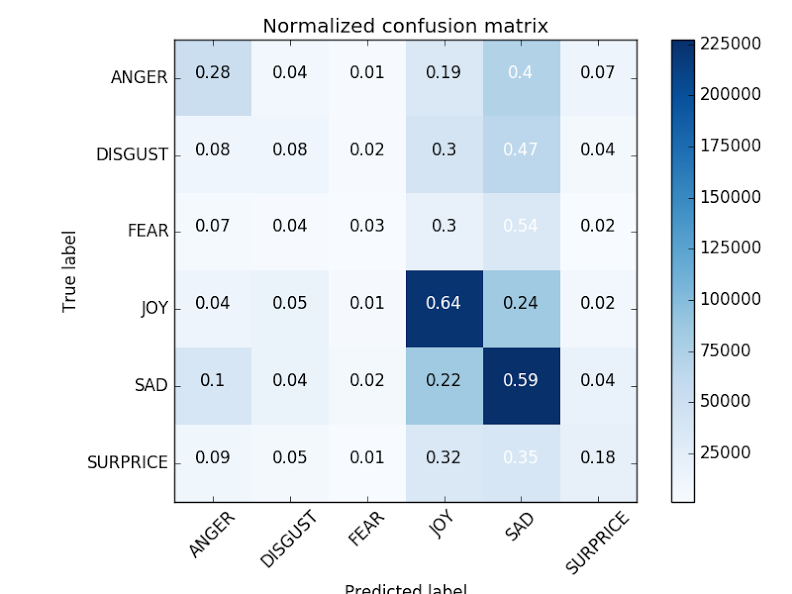
\includegraphics[width=1\linewidth]{tf-idf}
    \caption{The confusion matrix for TF-IDF+ SVM}
    \label{confusion1}
\end{figure}

\begin{figure}
\centering
\begin{subfigure}[b]{1\textwidth}
   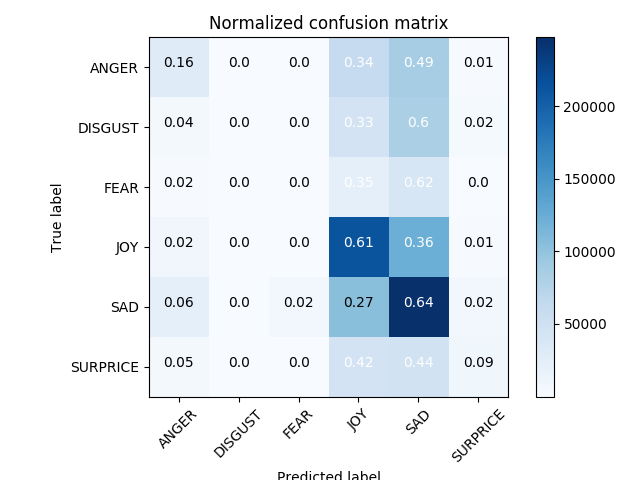
\includegraphics[width=.9\linewidth]{sc-ratio}
   \caption{}
   \label{confusion2} 
\end{subfigure}

\begin{subfigure}[b]{1\textwidth}
   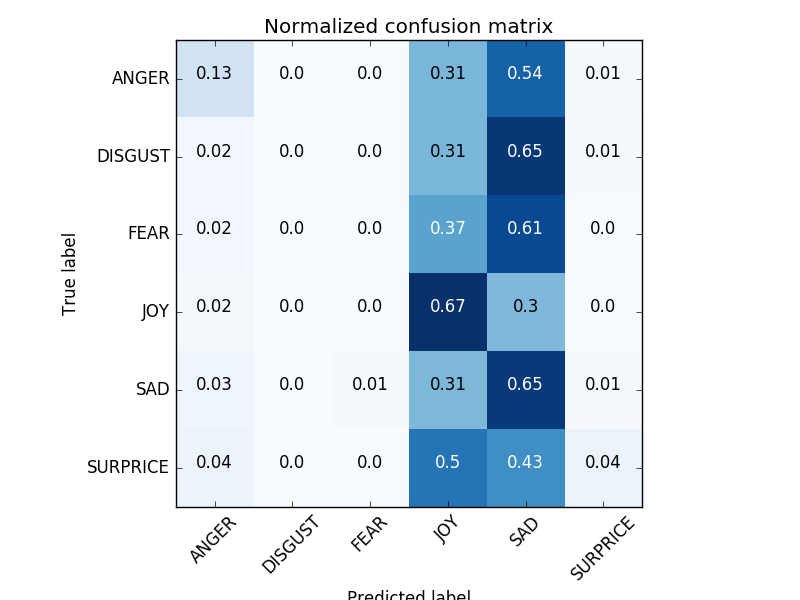
\includegraphics[width=.9\linewidth]{siamese-cbow-pretrained}
   \caption{}
   \label{confusion5}
\end{subfigure}
\caption[Confusion Matrix of Siamese-CBOW]{(a) The training set without pre-trained embedding,
(b) The training set with pre-trained embedding
}
\end{figure}


In the confusion matrix for FastText in Figure \ref{confusion4}, it shows different tendency for Pinyin dataset classification. 
The accuracy for SURPRISE is higher than SAD. It indicates that the SURPRISE may be modeled better than SAD, which contains more sample.
Figure \ref{confusion4} is quite similar with other confusion matrices, where most test data are classified as JOY and SAD.

\begin{figure}
\centering
\begin{subfigure}[b]{1\textwidth}
   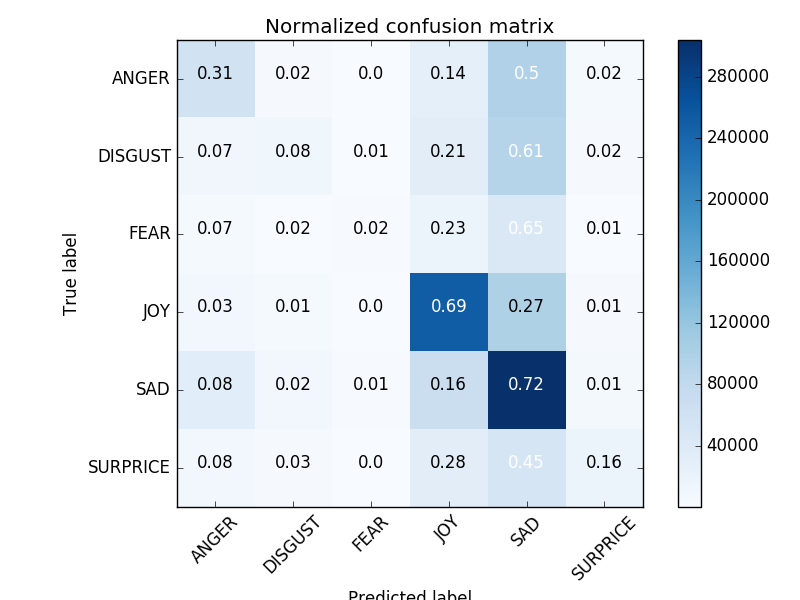
\includegraphics[width=.9\linewidth]{fasttext-All_seg_d300_w20_hs}
   \caption{}
   \label{confusion3} 
\end{subfigure}

\begin{subfigure}[b]{1\textwidth}
   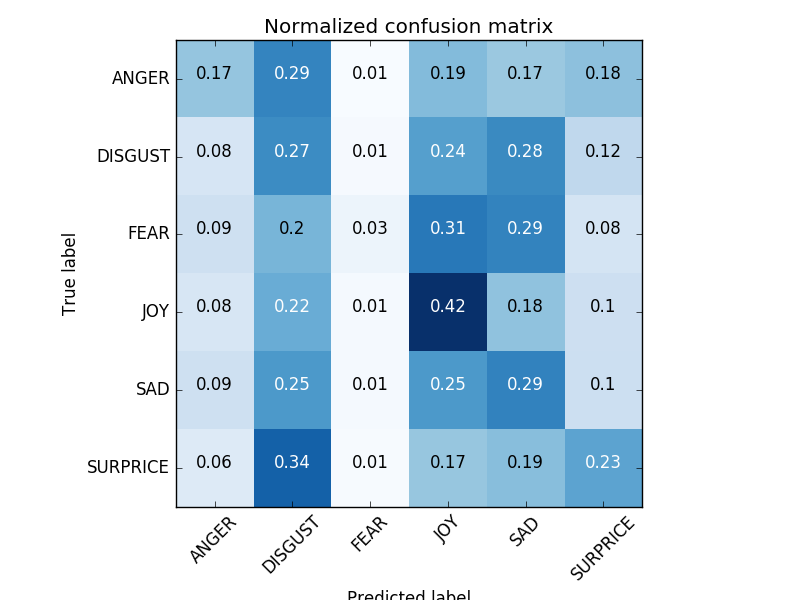
\includegraphics[width=.9\linewidth]{All_seg_d200_w15_softmax_pinyin}
   \caption{}
   \label{confusion4}
\end{subfigure}
\caption[Confusion matrix of FastText]{(a) segmented dataset trained with dimension=300, window size=20, loss function hierarchical softmax,
(b) pinyin dataset with dimension=200, window size=15, and loss function = softmax
}
\end{figure}
